\documentclass[handout]{beamer}

%%BEGIN HEADER
\usepackage{amsmath}
\usepackage{amssymb,amsthm,framed}
\usepackage{multirow,color,multicol}
\usepackage{fancyhdr,ifthen,lastpage}
\usepackage{verbatim,enumerate,cancel}
% --------------------------------------------------------------------
\newtheorem{thm}{Theorem}
\newtheorem{prop}{Proposition}

\theoremstyle{definition}
\newtheorem{defn}{Definition}
\newtheorem{fct}{Fact}

\theoremstyle{remark}
\newtheorem{remark}{Remark}

\newcommand{\Z}{\mathbb{Z}}
\newcommand{\C}{\mathbb{C}}
\newcommand{\Q}{\mathbb{Q}}
\newcommand{\N}{\mathbb{N}}
\newcommand{\R}{\mathbb{R}}
\newcommand{\B}{\mathcal{B}}
\renewcommand{\P}{\mathcal{P}}
\renewcommand{\L}{\mathcal{L}}
\newcommand{\F}{\mathbf{F}}
\newcommand{\x}{\mathbf{x}}
\newcommand{\y}{\mathbf{y}}

\newcommand{\sm}{\setminus}
\newcommand{\es}{\emptyset}
\newcommand{\ol}{\overline}
\newcommand{\inv}{^{-1}}
\newcommand{\seq}[1]{\{ {#1}_n\}}
\newcommand{\ds}{\displaystyle}
\newcommand{\mbf}{\mathbf}
\renewcommand{\=}{&=&}
\newcommand{\<}{\langle}
\renewcommand{\>}{\rangle}

\newcommand{\bmat}{\begin{bmatrix}}
\newcommand{\emat}{\end{bmatrix}}
\newcommand{\beq}{\begin{eqnarray*}}
\newcommand{\eeq}{\end{eqnarray*}}

\DeclareMathOperator{\repart}{Re}
\DeclareMathOperator{\impart}{Im}
\DeclareMathOperator{\Arg}{Arg}
\DeclareMathOperator{\trace}{tr}
\DeclareMathOperator{\rk}{rank}
\DeclareMathOperator{\nullsp}{null}
\DeclareMathOperator{\range}{range}
\DeclareMathOperator{\vspan}{span}
\DeclareMathOperator{\nullity}{nullity}

\setlength{\arraycolsep}{1cm}
%%%%%END HEADER

\mode<handout>
%\usetheme{Berlin}
%\usecolortheme{orchid}
 
\title{Lecture 8: Local Canonical Form}
\author{Prof. Weiqing Gu}
\date{}
\institute{Math 142:\\Differential Geometry}

%--------------------
\begin{document}
%--------------------
\small

%----------
\begin{frame}
\titlepage
\end{frame}

%----------
\begin{frame}[t]
\frametitle{Local Canonical Form}
\begin{block}{}
One of the most effective methods of solving problems in geometry consists of finding a coordinate
system which is adapted to the problem. In the study of local properties of a curve, in the
neighborhood of the point $s$, we have a natural coordinate system, namely the Frenet
trihedron at $s$. It is therefore convenient to refer the curve to this trihedron.
\end{block}
\begin{block}{}
Let $\alpha : I \to \R^3$ be a curve parametrized by arc length without singular points of order 1
(that is, $\alpha(s) \ne 0$ for all $s \in I$). We shall write the equations of the curve, in a
neighborhoods of $s_0$, using the trihedron $t(s_0)$, $n(s_0)$, $b(s_0)$ as a basis for $\R^3$.
\end{block}
\end{frame}

%----------
\begin{frame}[t]
\frametitle{Local Canonical Form}
\begin{block}{Equations}
Let us now take the system $0xyz$ in such a way that the origin 0 agrees with $\alpha(0)$ and
that $t = (1,0,0)$, $n = (0,1,0)$, and $b = (0,0,1)$. Under these conditions, $\alpha(s) = (x(s),y(s),
z(s))$ is given by
\begin{equation}
\label{LCF}
\begin{cases}
\ds x(s) = s - \frac{k^2 s^3}{6} + R_x, \\[5pt]
\ds y(s) = \frac{k s^2}{2} + \frac{k' s^3}{6} + R_y, \\[5pt]
\ds z(s) = -\frac{k \tau s^3}{6} + R_z,
\end{cases}
\end{equation}
where $R = (R_x, R_y, R_z)$. The representation (\ref{LCF}) is called the \emph{local canonical
form} of $\alpha$, in a neighborhood of $s = 0$.
\end{block}
\end{frame}

%----------
\begin{frame}[t]
\frametitle{A Sketch of projections of the trace of $\alpha$, for small $s$, in the $tn$, $tb$, and
$nb$ planes:}
\vspace{-.75cm}
\[
\begin{array}{cc}
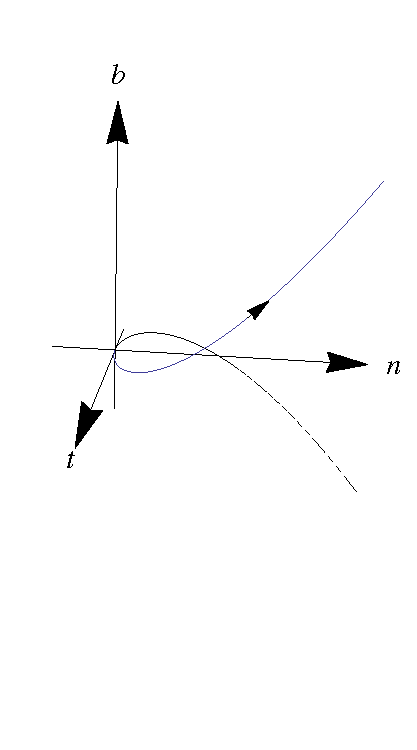
\includegraphics[scale=0.45]{ProjectionTemplate.pdf}
&  
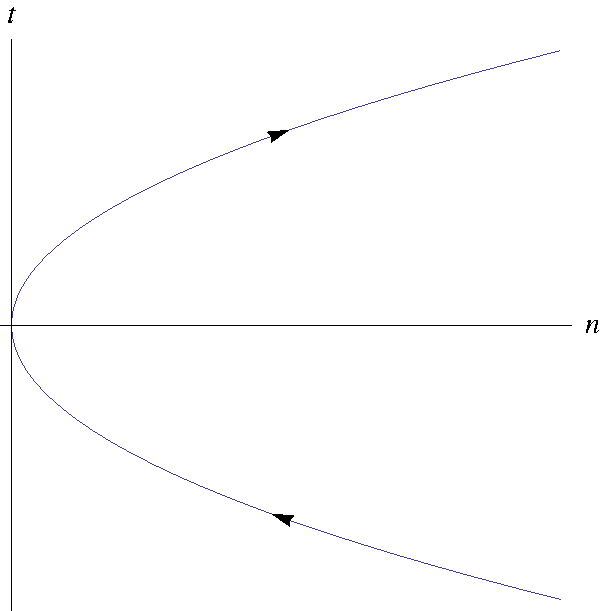
\includegraphics[scale=0.3]{ProjectionTN.pdf} 
\\
\text{{\tiny A Curve in $\R^3$}} & \text{{\tiny Projection over the plane $tn$}} \\
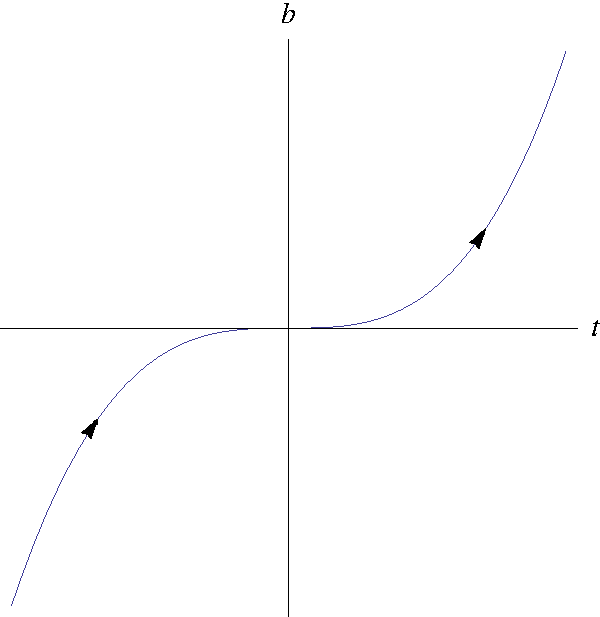
\includegraphics[scale=0.3]{ProjectionTB.pdf}
&
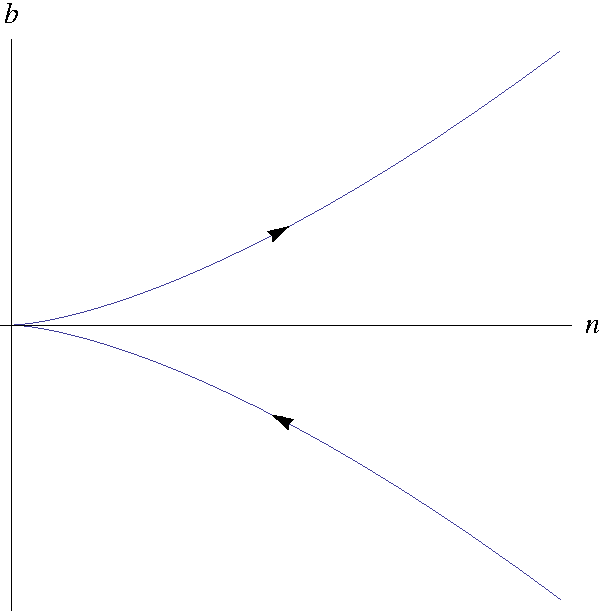
\includegraphics[scale=0.3]{ProjectionNB.pdf}\\
\text{{\tiny Projection over the plane $tb$}} & \text{{\tiny Projection over the plane $nb$}}
\end{array}
\]
\end{frame}

%----------
\begin{frame}[t]
\frametitle{Cautions and Subtleties}
\begin{center}
\large 1. We must distinguish a curve from its trace!
\end{center}
\begin{block}{Example}
The two distinct parametrized curves
\begin{align*}
\alpha(t) &= (\cos t, \sin t), \\
\beta(t) &= (\cos 2t, \sin 2t),
\end{align*}
where $t \in (0-\epsilon, 2\pi + \epsilon), \epsilon > 0$, have the same trace, namely, the circle
$x^2+y^2 = 1$. Notice that the velocity vector of the second curve is the double of the first one.
\end{block}
\end{frame}

%----------
\begin{frame}[t]
\frametitle{Cautions and Subtleties}
\begin{center}
\large 2. Changing the orientation of a curve.
\end{center}
\vfill
\begin{itemize}
\item Both curvature and torsion are invariant under the change of orientation, while the tangent
vector changes its orientation. The normal vector is invariant under a change of orientation and
the binormal changes orientation.
\end{itemize}
\end{frame}

%----------
\begin{frame}[t]
\frametitle{Cautions and Subtleties}
\begin{center}
3. $k(s) = 0 \Rightarrow \alpha(s)$ is a straight line (homework)\\
$\tau(s) \  \cancel{\Rightarrow} \  \alpha(s)$ is a plane curve.
\end{center}
\begin{block}{Example} \end{block}
\end{frame}

%----------
\begin{frame}[t]
\frametitle{Encouraged To Do}
\begin{block}{Do Carmo p. 25 \#10}
Consider the map
\[
\alpha(t) = \begin{cases} 
(t,0,e^{-1/t^2}), & t > 0 \\
(t,e^{-1/t^2},0), & t > 0 \\
(0,0,0), & t = 0
\end{cases}
\]
\vspace{-.5cm}
\begin{enumerate}[a.]
\item Prove that $\alpha$ is a differentiable curve
\item Prove that $\alpha$ is regular for all $t$ and that the curvature $k(t) \ne 0$ for $t \ne 0, t
\ne \pm \sqrt{2/3}$, and $k(0) = 0$.
\item Show that the limit of the osculating planes as $t \to 0$, $t > 0$, is the plane $y=0$ but that
the limit of the osculating planes as $t \to 0$, $t < 0$, is the plane $z=0$ (this implies that the
normal vector is discontinuous at $t = 0$ and shows why we excluded points where $k = 0$).
\item Show that $\tau$ can be defined so that $\tau = 0$, even though $\alpha$ is not a plane
curve.
\end{enumerate}
\end{block}
\end{frame}

%----------
\begin{frame}[t]
\frametitle{Cautions and Subtleties}
\begin{center}
\large 4. While $k(s) \ge 0$, $\tau(s)$ may be either positive or negative.
\end{center}
\vspace{-.75cm}
\begin{block}{}
From the third equation of (\ref{LCF}) it follows that if $\tau < 0$ and $s$ is sufficiently small,
then $z(s)$ increases with $s$. Let us make the convention of calling the ``positive side'' of the
osculating plane that side toward which $b$ is pointing. Then, since $z(0) = 0$, when we
describe the curve in the direction of increasing arc length, the curve will cross the osculating
plane at $s = 0$, pointing toward the positive side. If, on the contrary, $\tau > 0$, the curve
(described in the direction of increasing arc length) will cross the osculating plane pointing
to the side opposite the positive side.
\end{block}
\end{frame}

%----------
\begin{frame}[t]
\frametitle{Positive and Negative Torsion}
\begin{block}{Example}
The helix of Exercise 1 of Sec. 1-5 (Do Carmo) has negative torsion. An example of a curve with
positive torsion is the helix
\[
\alpha(s) = \left( a \cos \frac{s}{c}, a \sin \frac{s}{c}, -b\frac{s}{c}\right)
\]
obtained from the first one by a reflection in the $xz$ plane.
\end{block}
\pause
\begin{remark}
It is also usual to define torsion by $b' = - \tau n$. With such a definition, the torsion of the helix
of Exercise 1 becomes positive.
\end{remark}
\end{frame}

%----------
\begin{frame}[t]
\frametitle{Exercise Problems}
\begin{block}{Do Carmo pg. 47 \#2a}
Let $\alpha : I \to \R^3$ be a curve parametrized by arc length, with curvature $k(s) \ne 0$,
$s \in I$. Show that the osculating plane at $s$ is the limit position of the plane passing through
$\alpha(s)$, $\alpha(s+h_1)$, $\alpha(s+h_2)$ when $h_1, h_2 \to 0$.
\end{block}
\pause
\begin{solution}
Consider the local canonical form at $s$. Without loss of generality, we may assume that $s = 0$,
and we construct our coordinate system so that $e_1 = \vec t(0)$, $e_2 = \vec n(0)$, and $e_3 = 
\vec b(0)$.

\pause
\vspace{3mm}

Consider a plane passing through $\alpha(0)$, $\alpha(h_1)$, and $\alpha(h_2)$. 
Say the plane equation is $ax + by + cz = 0$. Here we may assume that the normal vector 
$$N = \bmat a \\ b \\ c \emat$$ 
to the plane is a unit vector.
\end{solution}
\end{frame}

%----------
\begin{frame}[t]
\frametitle{Exercise Problems}
\begin{solution}
Now for any point $\alpha(s)$ on the curve which is close to $\alpha(0)$, let us consider the length
$F(s)$ of the normal projection of $\alpha(s)$ to $N$. Then 
\begin{align} \label{proj} F(s) = \alpha(s) \cdot N = a x(s) + b y(s) + c z(s). \end{align}
Since $\alpha(h_1)$, $\alpha(h_2)$, and $\alpha(0)$ are on the plane, their projection to $N$ is
0. Hence, $F(0) = F(h_1) = F(h_2) = 0$.
\pause
\vspace{3mm}

By differentiating, we see that $F'(s) = \alpha'(s) \cdot N$. Therefore 
\begin{align} 
\label{deriv} 
F'(0) = \alpha'(0) \cdot N = t(0) \cdot N = (1,0,0) \cdot (a,b,c) = a. 
\end{align}
Similarly, $F''(s) = \alpha''(s) \cdot N$, so $F''(0) = k(0) b$.
\pause
\vspace{3mm}

\emph{Note:} You can also find $F'(s)$ by using local canonical form to calculate $x'(s), y'(s),$
and $z'(s)$ and get $x'(0) = 1, y'(0) = z'(0) = 0$. Similarly, to find $F''(s)$ you can find $x''(0) = 0$,
$y''(0) = k$, and $z''(0) = 0$.
\end{solution}
\end{frame}

%----------
\begin{frame}[t]
\frametitle{Exercise Problems}
\begin{solution}
However,
\[ 
F'(0) = \lim_{h_1 \to 0} \frac{\cancelto{0}{F(h_1)} - \cancelto {0}{F(0)}}{h_1} 
= \lim_{h_1 \to 0} \frac{0}{h_1} = 0,
\]
So by Equation (\ref{proj}), $a = 0$.
\pause
\vspace{3mm}

Similarly,
\[
F''(0) = \lim_{h_2 \to 0} \frac{F'(h_2)-F'(0)}{h_2} 
= \lim_{h_2 \to 0} \frac{\ds \lim_{h_1 \to h_2} \frac{\cancelto{0}{F(h_1)} - \cancelto{0}{F(h_2)}}
	{h_1 - h_2} - 0}{h_2}
= 0,
\]
so by Equation (\ref{deriv}), $k(0) b = 0$. Since $k(0) \ne 0$, it follows that $b = 0$.
\end{solution}
\end{frame}

%--------
\begin{frame}[t]
\frametitle{Exercise Problems}
\begin{solution}
Thus, as $h_1,h_2 \to 0$, the equation of the plane becomes $cz = 0$. Since $a^2+b^2+c^2=1$
by assumption, it follows that $c = \pm 1$. Therefore, the equation of the limit position of the
plane passing through $\alpha(0)$, $\alpha(h_1)$, $\alpha(h_2)$ is $z = 0$. Since this is precisely 
the osculating plane at $0$, the assertion holds.
\end{solution}
\end{frame}

%----------
\begin{frame}[t]
\frametitle{Exercise Problems}
\begin{block}{Do Carmo pg. 47 \#2b}
Let $\alpha : I \to \R^3$ be a curve parametrized by arc length, with curvature $k(s) \ne 0$,
$s \in I$. Show that the limit position of the circle passing through $\alpha(s)$, $\alpha(s+h_1)$,
$\alpha(s+h_2)$ when $h_1,h_2 \to 0$ is a circle in the osculating plane at $s$, the center of
which is on the line that contains $n(s)$ and the radius of which is the radius of curvature
$1/k(s)$; this circle is called the \emph{osculating circle} at $s$.
\end{block}
\pause
\begin{solution}
We have shown that the limit position of the plane $P_{h_1 h_2}$ passing through $\alpha(0)$,
$\alpha(h_1)$, and $\alpha(h_2)$ as $h_1,h_2 \to 0$ is the osculating plane $P$ at $s=0$. 
\pause\vspace{3mm}

If a circle passes through $\alpha(0)$, $\alpha(h_1)$, and $\alpha(h_2)$, then it must lie on the 
plane $P_{h_1 h_2}$. As $h_1, h_2 \to 0$, $P_{h_1 h_2} \to P$, so the circle $C_{h_1 h_2}$
tends to a limit circle $C$ in the plane $P$ with radius $r$. Note that $r$ could be 0.
\end{solution}
\end{frame}

%----------
\begin{frame}[t]
\frametitle{Exercise Problems}
\begin{solution}
Since the circle passes through the origin at $\alpha(0)$, we can write the circle's equation as
\[
	(x-x_0)^2 + (y-y_0)^2 = x_0^2 + y_0^2,
\]
or more simply,
\[
	x^2 - 2 x_0 x + y^2 - 2 y_0 y = 0.
\]
\pause \vspace{3mm}

Notice that, at $\alpha(0)$, the limiting circle and the curve have the same tangent. Let the circle
be parametrized by $h_1$:
\begin{align}
\label{param}
x(h_1)^2 - 2x_0 x(h_1) + y(h_1)^2 - 2y_0 y(h_1) = 0.
\end{align}
\end{solution}
\end{frame}

%----------
\begin{frame}[t]
\frametitle{Exercise Problems}
\begin{solution}
As $h_1$ approaches zero, the point on the circle can be viewed as the point on the curve up to
the derivative of order 1. Thus, by the local canonical form,
\begin{align}
\label{LCF2}
\begin{cases}
x(h_1) = h_1 - \frac{k^2}{6}h_1^3 + R_x \\
y(h_1) = \frac{k}{2} h_1^2 + \frac{k'}{6} h_1^3 + R_y \\
z(h_1) = -\frac{k \tau}{6} h_1^3 + R_z
\end{cases}
\end{align}
\pause

Plugging (\ref{LCF2}) into (\ref{param}), dividing both sides by $h_1$, and taking the limit as $h_1
\to 0$, we find that $x_0 = 0$. Hence, (\ref{param}) becomes
\begin{align} \label{param2}
x(h_1)^2 + y(h_1)^2 - 2y_0y(h_1) = 0.
\end{align}
\pause
Dividing both sides of (\ref{param2}) by $h_1^2$ and taking the limit as $h_1 \to 0$, we find that
$y_0 = 1/k$. Thus, the circle is centered on the $y$ axis (the line containing the $\vec n(s)$ by
construction) and has radius $1/k$, as desired.
\end{solution}
\end{frame}

%----------
\begin{frame}[t]
\frametitle{}

\end{frame}

%--------------------
\end{document}
%--------------------